\documentclass[a4paper,12pt]{article}

\usepackage[a4paper]{geometry}

\usepackage[utf8]{inputenc}            % Use utf8 input encoding
%\usepackage[latin1]{inputenc}         % Use iso 8859-1 encoding
\usepackage[T1]{fontenc}               % T1 fonts (support for accents/diacritics)
\usepackage{lmodern}                   % font with proper T1 support and good glyph quality

\usepackage{listings}                  % for (code) listings
\usepackage{amsmath}                   % AMS math typesetting
\usepackage{titlesec}
\usepackage{graphicx}
\usepackage{multirow}

\usepackage{hyperref}                  % better references for PDF

\titleformat{\section}{\LARGE\bfseries}% hide redundant number
            {}{0pt}{}

\begin{document}

\begin{center}
	\rule{\textwidth}{0.1pt}\\[1cm]
	
	\Large Softwarepraktikum SS 2018\\\bf Assignment 5 %EDIT
\end{center}


\begin{center}

	\rule{\textwidth}{0.1pt}\\[0.5cm]

	{\Large Group - 3\\[5mm]} %EDIT

	\begin{tabular}{lll}
		%EDIT
		Ramil Sabirov & 369500 & ramil.sabirov@rwth-aachen.de\\

		Joel Choi & 345575 & joel.choi@rwth-aachen.de \\

		Eric Remigius & 366895 & eric.remigius@rwth-aachen.de \\

	\end{tabular}\\[0.5cm]

	\rule{\textwidth}{0.1pt}\\[1cm]

\end{center}

% Uncomment next two lines for table of contents !not needed!
%\newpage
%\tableofcontents

\section*{Task 1}
An dieser Stelle wollen wir auf das Assignment 3 verweisen. Dort wurde bereits unsere Zeitschätzung für die nächste Tiefe erläutert.\\
Kurzgefasst: Wir wählen sehr konservativ den maximalen Verzweigungsgrad des Variantenbaumes als Faktor für die nächste Tiefe. Damit gehen wir nahezu allen möglichen Timeouts aus dem Weg. Jedoch beenden Spiele wir auch des öfteren mit einem riesigen Zeitkonto, welches dann verschwendet ist.
\section{Task 2}
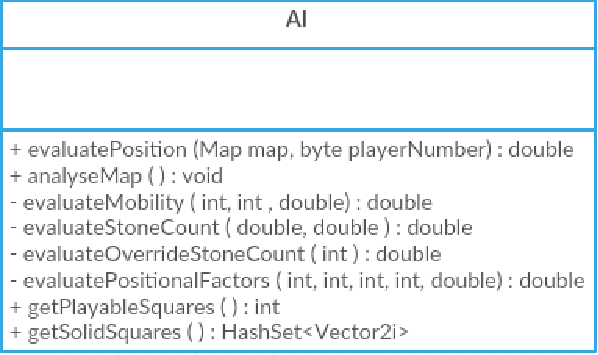
\includegraphics[scale=0.5]{AIClassdiagram.pdf}
Unsere Bewertungsfunktion behandelt verschiedene Aspekte des Spieles. Diese wären:
\begin{enumerate}
\item[-] Stabile Felder
\item[-] Feldkontrolle
\item[-] Mobilität (Anzahl "kostenfreier" Züge)
\item[-] Anzahl Overridesteine
\end{enumerate}
Dabei geht die Evaluationsfunktion für jede dieser Eigenschaften ähnlich vor: 
\begin{enumerate}
\item[1.] Bestimme den erwarteten Wert der Eigenschaft für die aktuelle Spielsituation
\item[2.] Multipliziere die Differenz zum realen Wert mit einem Bonusfaktor
\item[3.] Skaliere den errechneten Wert mit einer Wichtigkeitsfunktion abhängig von aktueller Spielsituation (Meistens das Stadium des Spieles)
\end{enumerate}
Die Wichtigkeitsfunktionen $$w_i:\ [0,1] \rightarrow [0,1]$$ legen demnach fest wie viel Einfluss eine Eigenschaft zu dem konkreten Zeitpunkt hat auf die Evaluation hat. Zum Beispiel ist die Anzahl der eigenen Steine (Feldkontrolle) am Anfang des Spieles nahezu unwesentlich und zum Ende hin das Einzige was zählt:
\begin{center}
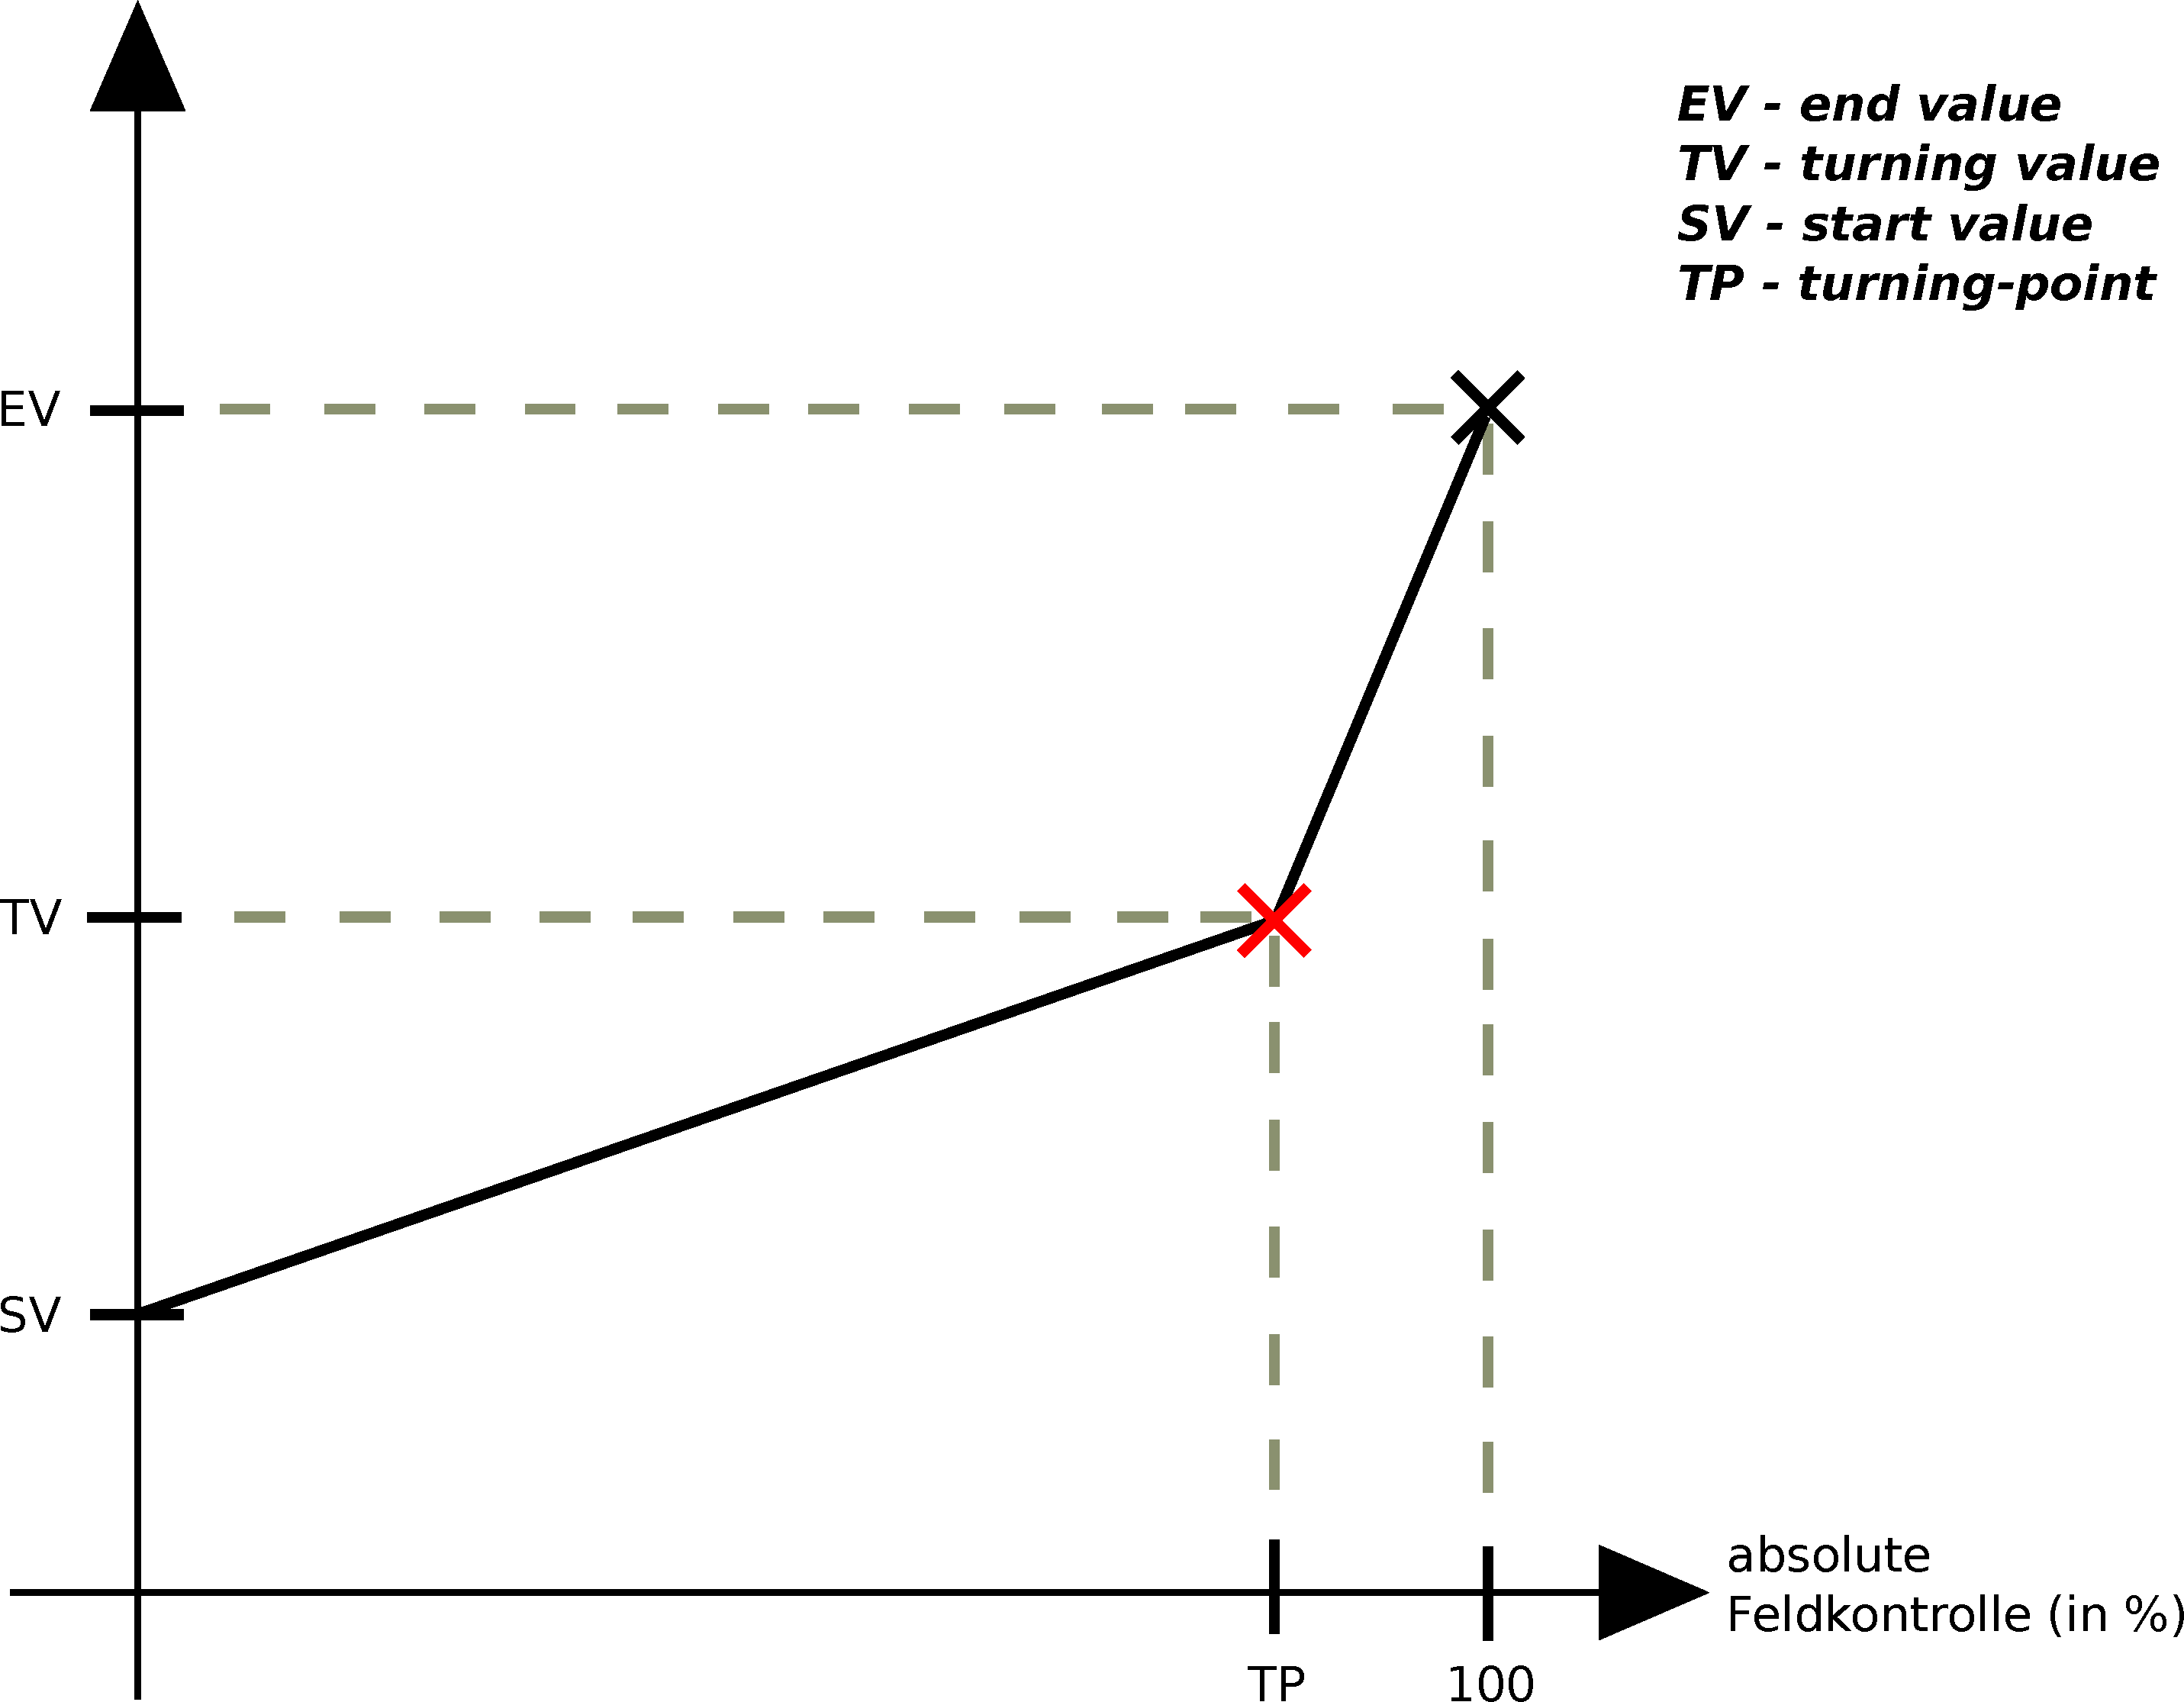
\includegraphics[scale=0.15]{ImportanceFunctionGraph.pdf}
\end{center}
Durch einfache lineare Approximation der Wichtigkeit, verlieren wir den sanften Übergang zwischen den Phasen vor und nach dem Wendepunkt. Jedoch beugen wir mögliche Überanpassung vor, welche starke Schwankungen der Funktion in manchen Bereichen zur Folge haben könnte und die Bewertung zum "Zittern" bringen würde.\\
Ähnlich sieht die Funktion aus für die stabilen Felder. Diese ist jedoch monoton fallend $SV \geq TV \geq EV$, da positionelles Spiel zum Ende hin vom konkreten Spiel verdrängt wird. Weil Mobilität stets wichtig ist, sowohl am Ende als auch am Anfang, weicht diese Wichtigkeitsfunktion ab und betrachtet die Anzahl der Spielzüge, bis man wieder selber an der Reihe ist. Die Anzahl der Overridesteine hat aus demselben Grund die Wichtigkeit konstant 1.\\\\
Die Funktionen für den erwartenden Wert sind grundsätzlich dazu da, dass sich die Stellungsbewertung nicht grundlos verbessert oder verschlechtert. So ist z.B. die Mobilität am Anfang des Spieles eingeschränkt, da noch nicht genug Steine auf dem Feld liegen. Steigt auf natürliche Art und Weise an im Laufe des Spieles und nimmt wieder ab zum Ende, da die meisten Felder belegt sind. Ignoriert man den Verlauf, verbessert sich natürlicherweise die eigene Bewertung am Anfang des Spieles (ohne etwas besonders Gutes leisten zu müssen) und verschlechtert sich zum Ende hin, auch wenn man vielleicht stark spielt. Unsere Modellierung der Mobilität ist dementsprechend:
\begin{center}
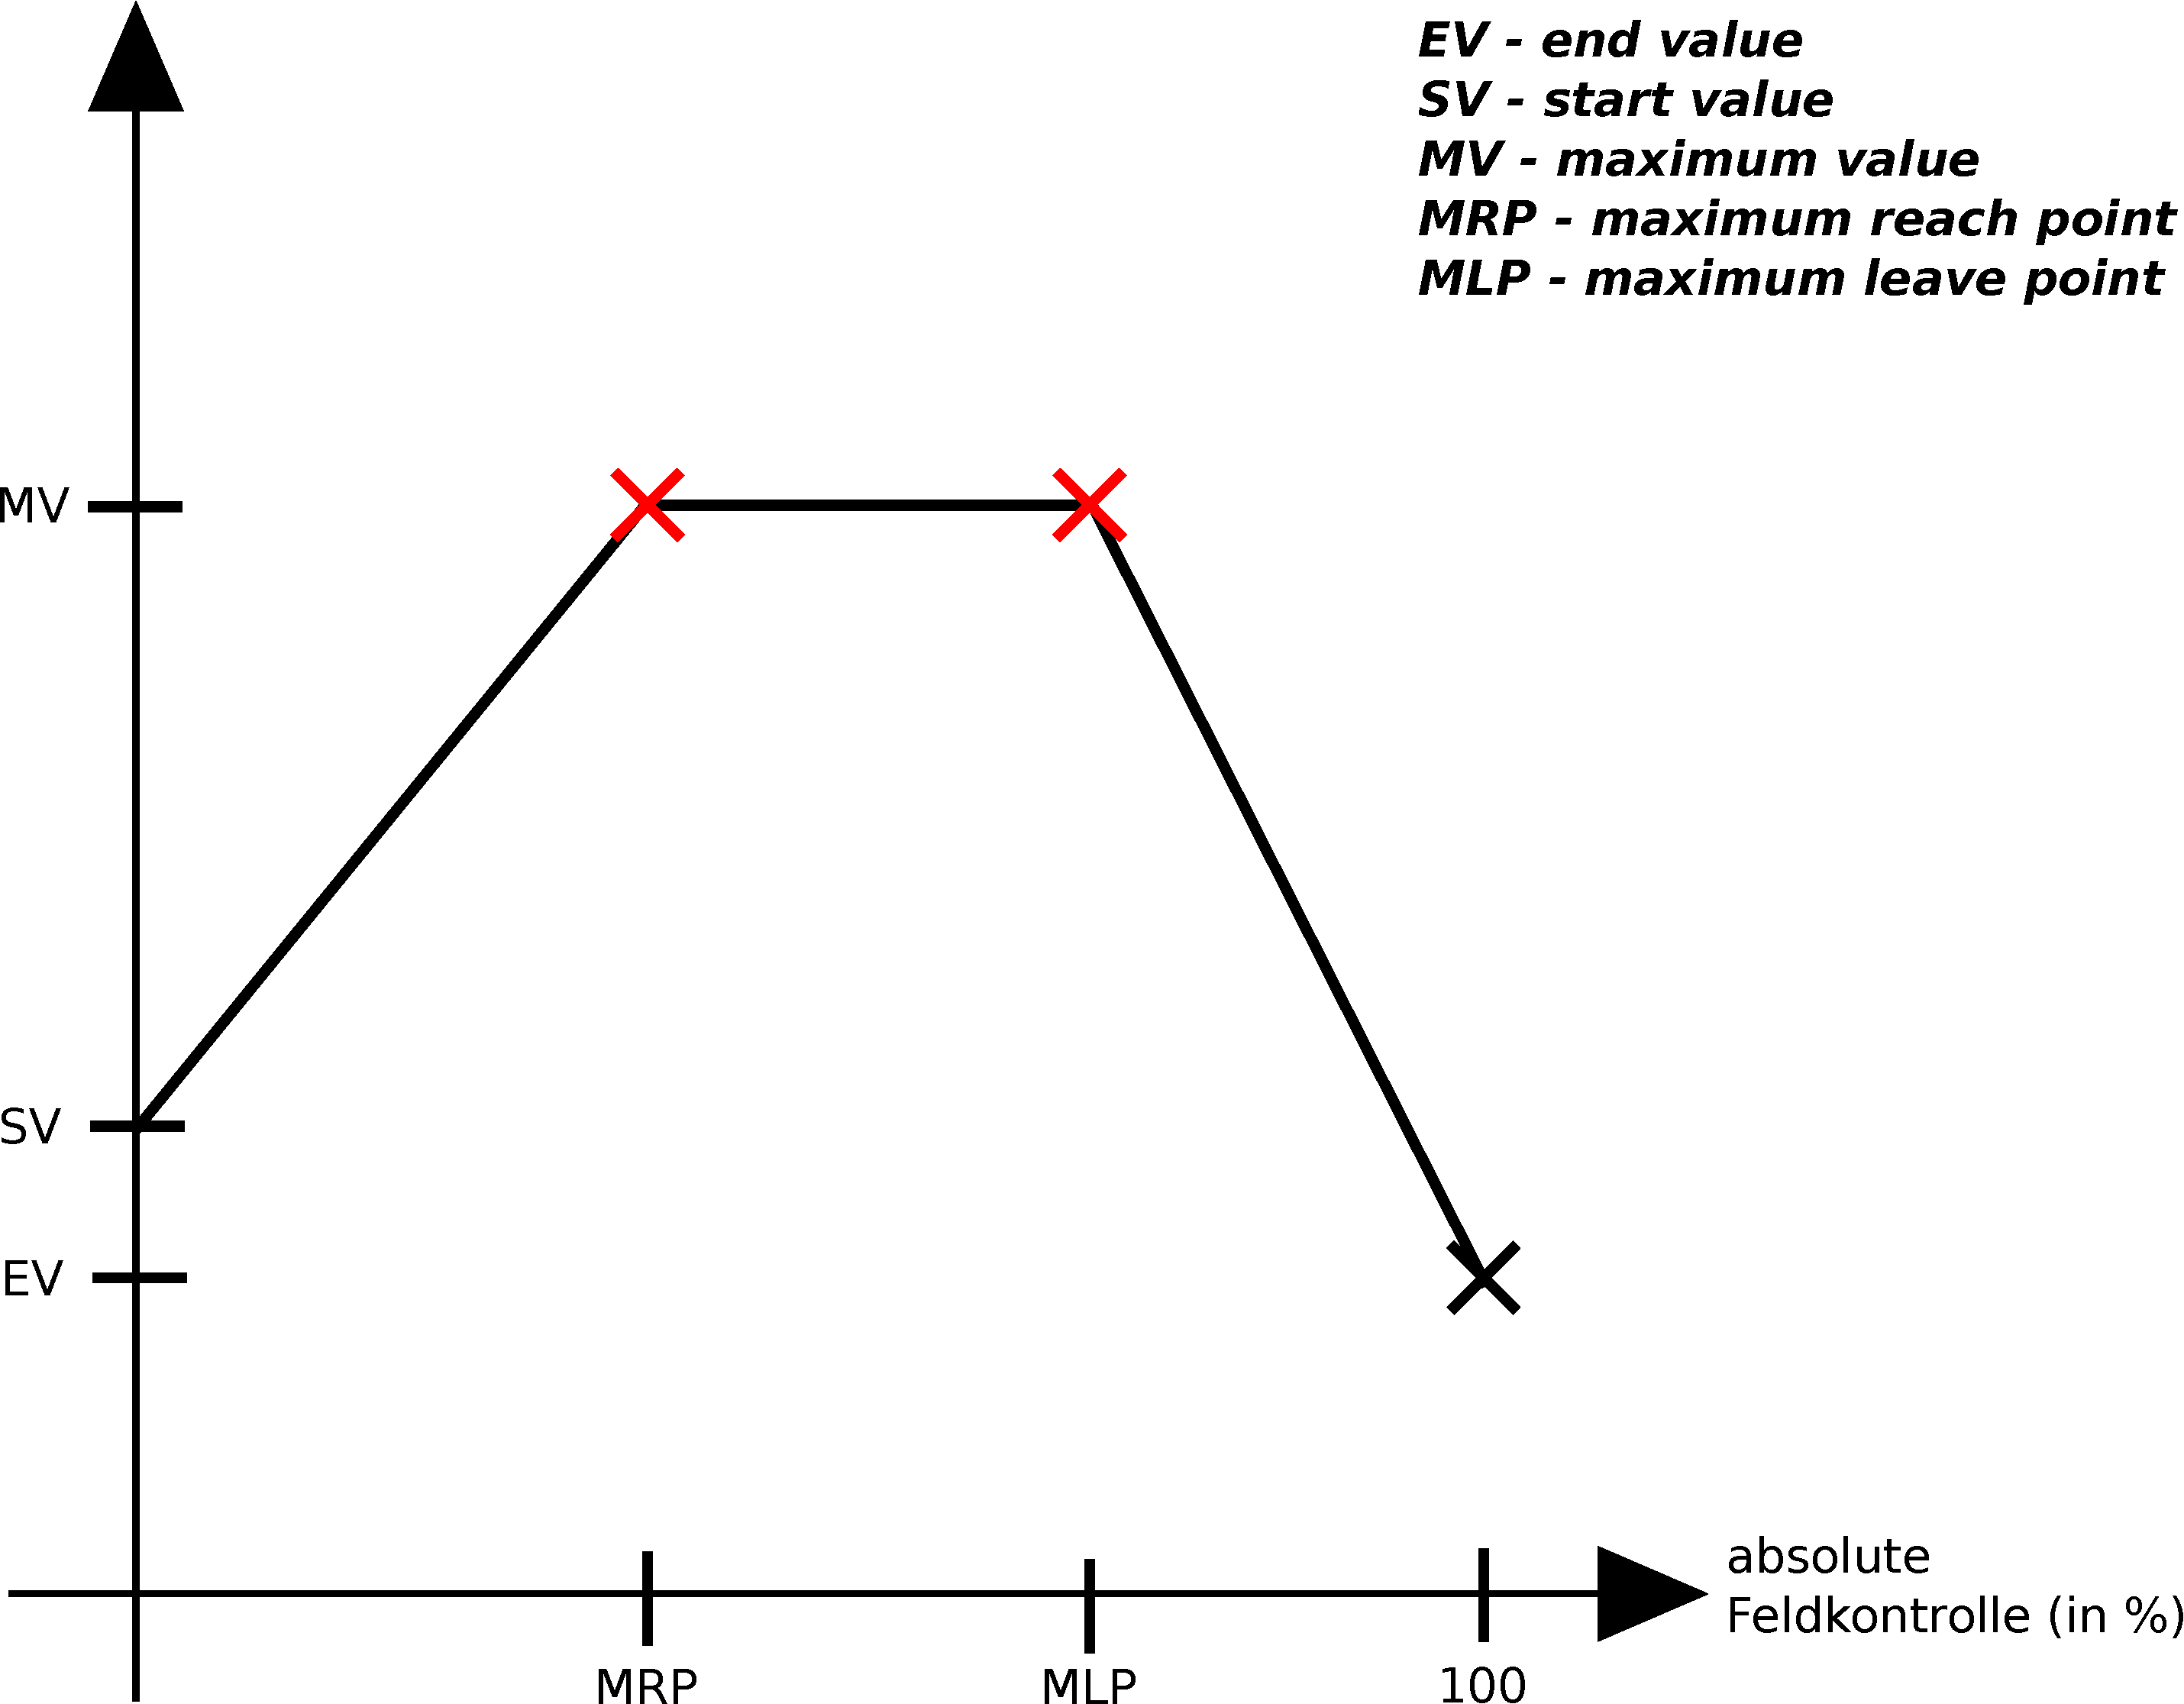
\includegraphics[scale=0.15]{ExpectedValueFunction.pdf}
\end{center}
Die Funktionen für die Anzahl der Overridesteine und stabilen Felder ist zunächst konstant 0 gelassen, aufgrund mangelnder Erfahrung und Einschätzbarkeit. Die Funktion für die eigene Feldkontrolle nimmt einen ähnlichen Verlauf wie die Wichtigkeitsfunktion.\\
Mit der hohen Parametrisierung erhoffen wir uns eine hohe und systematische Anpassbarkeit der Bewertungsfunktion. Mit steigender Spielerfahrung sollten sich gute heuristische Werte einpendeln.
\newline

\noindent
Nun haben wir auch die Methode anlayseMap, die schaut auf der ganzen Map schaut, ob es stabile Felder gibt und diese im HashSet solidSquares speichert. Die Methode iteriert über die ganze Map und schaut bei Feldern, die keine Löcher sind, ob diese stabil sind, indem man schaut ob alle 4 Richtungen blockiert sind. Ausserdem wird beim iterieren über der Map alle bespielbaren Felder mit dem Counter playableSquares gezählt.


\section{Task 3}
Um einen möglichst großen Gewinn in der Performance zu erzielen, müssen wir versuchen, die \textit{Aspiration-Windows} möglichst klein zu halten, damit viele Zweige abgeschnitten werden.

Da unsere Bewertungsfunktion uns einen Wert zwischen 0 und 250 liefert, kann die Größe des Fensters maximal 250 groß sein. Aber wir wollen ja ein möglichst kleines Fenster haben. Deshalb haben wir zuerst auf der Standard Karte eine Binäre Suche ausgeführt, und haben festgestellt, dass erst ab einer Größe von ca. 15-20 die oben beschriebenen \textit{Aspiration-Window Fails} auftreten.

Um diesen Wert besser ausfeilen zu können, haben wir ein Script geschrieben, dass auf fünf Karten je sieben Spiele spielt und dabei die folgenden Fenstergrößen ausprobiert:

$$ 50, 40, 30, 20, 15, 10, 5$$

Dabei haben wir festgestellt, dass auf verschiedenen Karten die Schwelle, ab der \textit{Aspiration-Window Fails} auftreten, unterschiedlich ist. Somit macht es keinen Großen Sinn, die optimale Fenstergröße exakt zu bestimmen und eine Auflösung von 5 sollte genügen.

Die genauen Ergebnisse können in der Datei Aspiration-Ergebnisse.txt eingesehen werden.
Hier deshalb nur die wichtigsten Eckdaten:

\begin{tabular}{|c|c|c|}
\hline 
Map & Aspiration Window Size & Fails \\ 
\hline 
\hline
\multirow{3}{*}{standard\_map.txt} & 20 & 0  \\
                                   & 15 & 3  \\ 
                                   & 10 & 20 \\ 
\hline 

\multirow{3}{*}{005\_g5\_map2.txt} & 20 & 1 \\ 
                                   & 15 & 9 \\ 
                                   & 10 & 5 \\ 
\hline 

\multirow{3}{*}{006\_g6\_question\_mark.map} & 20 & 0 \\
                                             & 15 & 2 \\ 
                                             & 10 & 2 \\ 
\hline 

\multirow{3}{*}{009\_g7\_Map\_Pirate\_Heist} & 20 & 6 \\
                                             & 15 & 10 \\ 
                                             & 10 & 24 \\ 
\hline 
 
\multirow{3}{*}{011\_g3\_Map1.txt} & 20 & 0 \\
                                   & 15 & 0 \\ 
                                   & 10 & 0 \\ 
\hline 
\end{tabular} 

Da ein \textit{Aspiration-Window Fail} dazu führt, dass eine Suche erneut gestartet wird, kann es, vor allem in großen Tiefen, sehr teuer sein, weshalb wir den optimalen Wert sehr konservativ entschieden haben. 

Dieser optimale Wert ist für uns: 15

Auf allen getesteten Maps führt dieser Wert dazu, dass weniger als 0,03\% der Suchen fehlschlagen. Der nächst bessere Wert von 10 hätte auf einigen der Karten diese Grenze überschritten. Insgesamt denken wir also, dass es ein guter Kompromiss ist.

\end{document}
